\documentclass{standalone}
\usepackage{tikz}
\usetikzlibrary{patterns, positioning}


\begin{document}
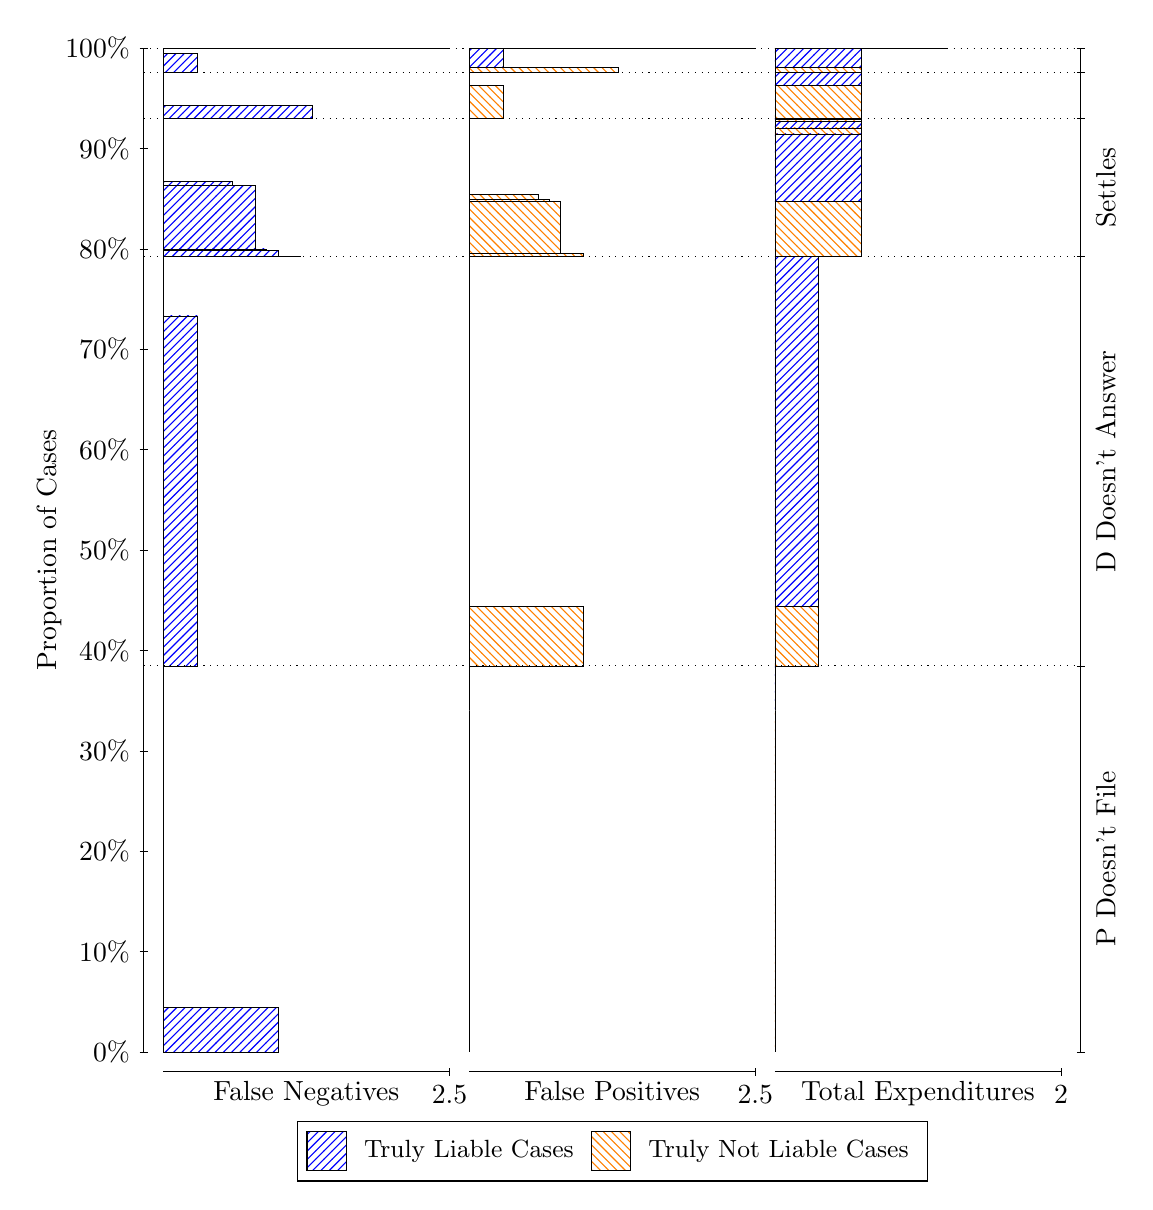
\begin{tikzpicture}
\draw[black, very thin] (1.5,1.75) -- (1.5,14.5);
\node[rotate=90, text=black, anchor=center] at (0.3, 8.125) {Proportion of Cases};
\draw[black, very thin] (1.45,1.75) -- (1.55,1.75);
\node[text=black, anchor=east] at (1.45, 1.75) {0\%};
\draw[black, very thin] (1.45,3.025) -- (1.55,3.025);
\node[text=black, anchor=east] at (1.45, 3.025) {10\%};
\draw[black, very thin] (1.45,4.3) -- (1.55,4.3);
\node[text=black, anchor=east] at (1.45, 4.3) {20\%};
\draw[black, very thin] (1.45,5.575) -- (1.55,5.575);
\node[text=black, anchor=east] at (1.45, 5.575) {30\%};
\draw[black, very thin] (1.45,6.85) -- (1.55,6.85);
\node[text=black, anchor=east] at (1.45, 6.85) {40\%};
\draw[black, very thin] (1.45,8.125) -- (1.55,8.125);
\node[text=black, anchor=east] at (1.45, 8.125) {50\%};
\draw[black, very thin] (1.45,9.4) -- (1.55,9.4);
\node[text=black, anchor=east] at (1.45, 9.4) {60\%};
\draw[black, very thin] (1.45,10.675) -- (1.55,10.675);
\node[text=black, anchor=east] at (1.45, 10.675) {70\%};
\draw[black, very thin] (1.45,11.95) -- (1.55,11.95);
\node[text=black, anchor=east] at (1.45, 11.95) {80\%};
\draw[black, very thin] (1.45,13.225) -- (1.55,13.225);
\node[text=black, anchor=east] at (1.45, 13.225) {90\%};
\draw[black, very thin] (1.45,14.5) -- (1.55,14.5);
\node[text=black, anchor=east] at (1.45, 14.5) {100\%};

\draw[black, very thin] (13.4,1.75) -- (13.4,14.5);
\draw[black, very thin] (13.35,1.75) -- (13.45,1.75);
\node[anchor=west] at (13.35, 1.75) {};
\draw[black, very thin] (13.35,6.6537) -- (13.45,6.6537);
\node[anchor=west] at (13.35, 6.6537) {};
\draw[black, very thin] (13.35,11.849) -- (13.45,11.849);
\node[anchor=west] at (13.35, 11.849) {};
\draw[black, very thin] (13.35,13.603) -- (13.45,13.603);
\node[anchor=west] at (13.35, 13.603) {};
\draw[black, very thin] (13.35,14.194) -- (13.45,14.194);
\node[anchor=west] at (13.35, 14.194) {};
\draw[black, very thin] (13.35,14.494) -- (13.45,14.494);
\node[anchor=west] at (13.35, 14.494) {};
\draw[black, very thin] (13.35,14.497) -- (13.45,14.497);
\node[anchor=west] at (13.35, 14.497) {};
\draw[black, very thin] (13.35,14.5) -- (13.45,14.5);
\node[anchor=west] at (13.35, 14.5) {};

\draw[black, very thin, pattern color=blue, pattern=north east lines] (1.75,1.75) rectangle (3.2033,2.3163);
\draw[black, very thin, pattern color=orange, pattern=north west lines] (1.75,2.3163) rectangle (1.75,6.6537);
\draw[black, very thin, pattern color=blue, pattern=north east lines] (1.75,6.6537) rectangle (2.186,11.097);
\draw[black, very thin, pattern color=orange, pattern=north west lines] (1.75,11.097) rectangle (1.75,11.849);
\draw[black, very thin, pattern color=blue, pattern=north east lines] (1.75,11.849) rectangle (3.494,11.852);
\draw[black, very thin, pattern color=blue, pattern=north east lines] (1.75,11.852) rectangle (3.2033,11.932);
\draw[black, very thin, pattern color=blue, pattern=north east lines] (1.75,11.932) rectangle (3.058,11.936);
\draw[black, very thin, pattern color=blue, pattern=north east lines] (1.75,11.936) rectangle (3.058,11.949);
\draw[black, very thin, pattern color=blue, pattern=north east lines] (1.75,11.949) rectangle (2.9127,12.753);
\draw[black, very thin, pattern color=blue, pattern=north east lines] (1.75,12.753) rectangle (2.622,12.806);
\draw[black, very thin, pattern color=orange, pattern=north west lines] (1.75,12.806) rectangle (1.75,13.603);
\draw[black, very thin, pattern color=blue, pattern=north east lines] (1.75,13.603) rectangle (3.6393,13.767);
\draw[black, very thin, pattern color=orange, pattern=north west lines] (1.75,13.767) rectangle (1.75,14.194);
\draw[black, very thin, pattern color=blue, pattern=north east lines] (1.75,14.194) rectangle (2.186,14.434);
\draw[black, very thin, pattern color=orange, pattern=north west lines] (1.75,14.434) rectangle (1.75,14.494);
\draw[black, very thin, pattern color=blue, pattern=north east lines] (1.75,14.494) rectangle (5.3833,14.496);
\draw[black, very thin, pattern color=orange, pattern=north west lines] (1.75,14.496) rectangle (1.75,14.497);
\draw[black, very thin, pattern color=orange, pattern=north west lines] (1.75,14.497) rectangle (1.75,14.498);
\draw[black, very thin, pattern color=blue, pattern=north east lines] (1.75,14.498) rectangle (1.75,14.5);
\draw[black, very thin, pattern color=orange, pattern=north west lines] (5.6333,1.75) rectangle (5.6333,6.0874);
\draw[black, very thin, pattern color=blue, pattern=north east lines] (5.6333,6.0874) rectangle (5.6333,6.6537);
\draw[black, very thin, pattern color=orange, pattern=north west lines] (5.6333,6.6537) rectangle (7.0867,7.4056);
\draw[black, very thin, pattern color=blue, pattern=north east lines] (5.6333,7.4056) rectangle (5.6333,11.849);
\draw[black, very thin, pattern color=orange, pattern=north west lines] (5.6333,11.849) rectangle (7.0867,11.891);
\draw[black, very thin, pattern color=orange, pattern=north west lines] (5.6333,11.891) rectangle (6.796,12.554);
\draw[black, very thin, pattern color=orange, pattern=north west lines] (5.6333,12.554) rectangle (6.6507,12.574);
\draw[black, very thin, pattern color=orange, pattern=north west lines] (5.6333,12.574) rectangle (6.5053,12.64);
\draw[black, very thin, pattern color=orange, pattern=north west lines] (5.6333,12.64) rectangle (6.2147,12.646);
\draw[black, very thin, pattern color=blue, pattern=north east lines] (5.6333,12.646) rectangle (5.6333,13.603);
\draw[black, very thin, pattern color=orange, pattern=north west lines] (5.6333,13.603) rectangle (6.0693,14.029);
\draw[black, very thin, pattern color=blue, pattern=north east lines] (5.6333,14.029) rectangle (5.6333,14.194);
\draw[black, very thin, pattern color=orange, pattern=north west lines] (5.6333,14.194) rectangle (7.5227,14.254);
\draw[black, very thin, pattern color=blue, pattern=north east lines] (5.6333,14.254) rectangle (6.0693,14.494);
\draw[black, very thin, pattern color=orange, pattern=north west lines] (5.6333,14.494) rectangle (5.6333,14.496);
\draw[black, very thin, pattern color=blue, pattern=north east lines] (5.6333,14.496) rectangle (5.6333,14.497);
\draw[black, very thin, pattern color=orange, pattern=north west lines] (5.6333,14.497) rectangle (9.2667,14.498);
\draw[black, very thin, pattern color=blue, pattern=north east lines] (5.6333,14.498) rectangle (7.8133,14.5);
\draw[black, very thin, pattern color=orange, pattern=north west lines] (9.5167,1.75) rectangle (9.5167,6.0874);
\draw[black, very thin, pattern color=blue, pattern=north east lines] (9.5167,6.0874) rectangle (9.5167,6.6537);
\draw[black, very thin, pattern color=orange, pattern=north west lines] (9.5167,6.6537) rectangle (10.062,7.4056);
\draw[black, very thin, pattern color=blue, pattern=north east lines] (9.5167,7.4056) rectangle (10.062,11.849);
\draw[black, very thin, pattern color=orange, pattern=north west lines] (9.5167,11.849) rectangle (10.607,12.554);
\draw[black, very thin, pattern color=blue, pattern=north east lines] (9.5167,12.554) rectangle (10.607,13.411);
\draw[black, very thin, pattern color=orange, pattern=north west lines] (9.5167,13.411) rectangle (10.607,13.486);
\draw[black, very thin, pattern color=blue, pattern=north east lines] (9.5167,13.486) rectangle (10.607,13.573);
\draw[black, very thin, pattern color=orange, pattern=north west lines] (9.5167,13.573) rectangle (10.607,13.589);
\draw[black, very thin, pattern color=blue, pattern=north east lines] (9.5167,13.589) rectangle (10.607,13.603);
\draw[black, very thin, pattern color=orange, pattern=north west lines] (9.5167,13.603) rectangle (10.607,14.029);
\draw[black, very thin, pattern color=blue, pattern=north east lines] (9.5167,14.029) rectangle (10.607,14.194);
\draw[black, very thin, pattern color=orange, pattern=north west lines] (9.5167,14.194) rectangle (10.607,14.254);
\draw[black, very thin, pattern color=blue, pattern=north east lines] (9.5167,14.254) rectangle (10.607,14.494);
\draw[black, very thin, pattern color=orange, pattern=north west lines] (9.5167,14.494) rectangle (11.697,14.496);
\draw[black, very thin, pattern color=blue, pattern=north east lines] (9.5167,14.496) rectangle (11.697,14.497);
\draw[black, very thin, pattern color=orange, pattern=north west lines] (9.5167,14.497) rectangle (11.697,14.498);
\draw[black, very thin, pattern color=blue, pattern=north east lines] (9.5167,14.498) rectangle (11.697,14.5);
\draw[black, dotted] (1.5,6.6537) -- (13.4,6.6537);
\draw[black, dotted] (1.5,11.849) -- (13.4,11.849);
\draw[black, dotted] (1.5,13.603) -- (13.4,13.603);
\draw[black, dotted] (1.5,14.194) -- (13.4,14.194);
\draw[black, dotted] (1.5,14.494) -- (13.4,14.494);
\draw[black, dotted] (1.5,14.497) -- (13.4,14.497);
\draw[black, very thin] (1.75,1.5) -- (5.3833,1.5);
\node[text=black, anchor=north] at (3.5667, 1.5) {False Negatives};
\draw[black, very thin] (5.3833,1.45) -- (5.3833,1.55);
\node[text=black, anchor=north] at (5.3833, 1.45) {2.5};

\draw[black, very thin] (5.6333,1.5) -- (9.2667,1.5);
\node[text=black, anchor=north] at (7.45, 1.5) {False Positives};
\draw[black, very thin] (9.2667,1.45) -- (9.2667,1.55);
\node[text=black, anchor=north] at (9.2667, 1.45) {2.5};

\draw[black, very thin] (9.5167,1.5) -- (13.15,1.5);
\node[text=black, anchor=north] at (11.333, 1.5) {Total Expenditures};
\draw[black, very thin] (13.15,1.45) -- (13.15,1.55);
\node[text=black, anchor=north] at (13.15, 1.45) {2};

\node[text=black, centered, rotate=90] at (13.72, 4.2019) {P Doesn't File};
\node[text=black, centered, rotate=90] at (13.72, 9.2515) {D Doesn't Answer};
\node[text=black, centered, rotate=90] at (13.72, 12.726) {Settles};





\draw (7.449999999999999,1.5) node[draw=none] (baseCoordinate) {};
\begin{scope}[align=center]
        \matrix[scale=0.5, draw=black, below=0.5cm of baseCoordinate, nodes={draw}, column sep=0.1cm]{
            \node[rectangle, draw, minimum width=0.5cm, minimum height=0.5cm, pattern color=blue, pattern=north east lines] {}; &
            \node[draw=none, font=\small, text=black] (B) {Truly Liable Cases}; &
            \node[rectangle, draw, minimum width=0.5cm, minimum height=0.5cm, pattern color=orange, pattern=north west lines] {}; &
            \node[draw=none, font=\small, text=black] (B) {Truly Not Liable Cases}; \\
            };
\end{scope}

\end{tikzpicture}
\end{document}